\documentclass[]{scrartcl}
\usepackage{graphicx}

%opening
\title{Demo OFC 2018 - Workflow}
\author{Javier Moreno Muro}

\begin{document}

\maketitle


\section{Objective}

In a metro network with VIMs orchestrated by an ETSI-OSM instance, and an optical transport controller, we demonstrate optimized service chain provisioning using the open-source Net2Plan tool with interfaces to OSM (new) and transport controller

\begin{figure}[h!]
	\centering
	\label{fig:original}
	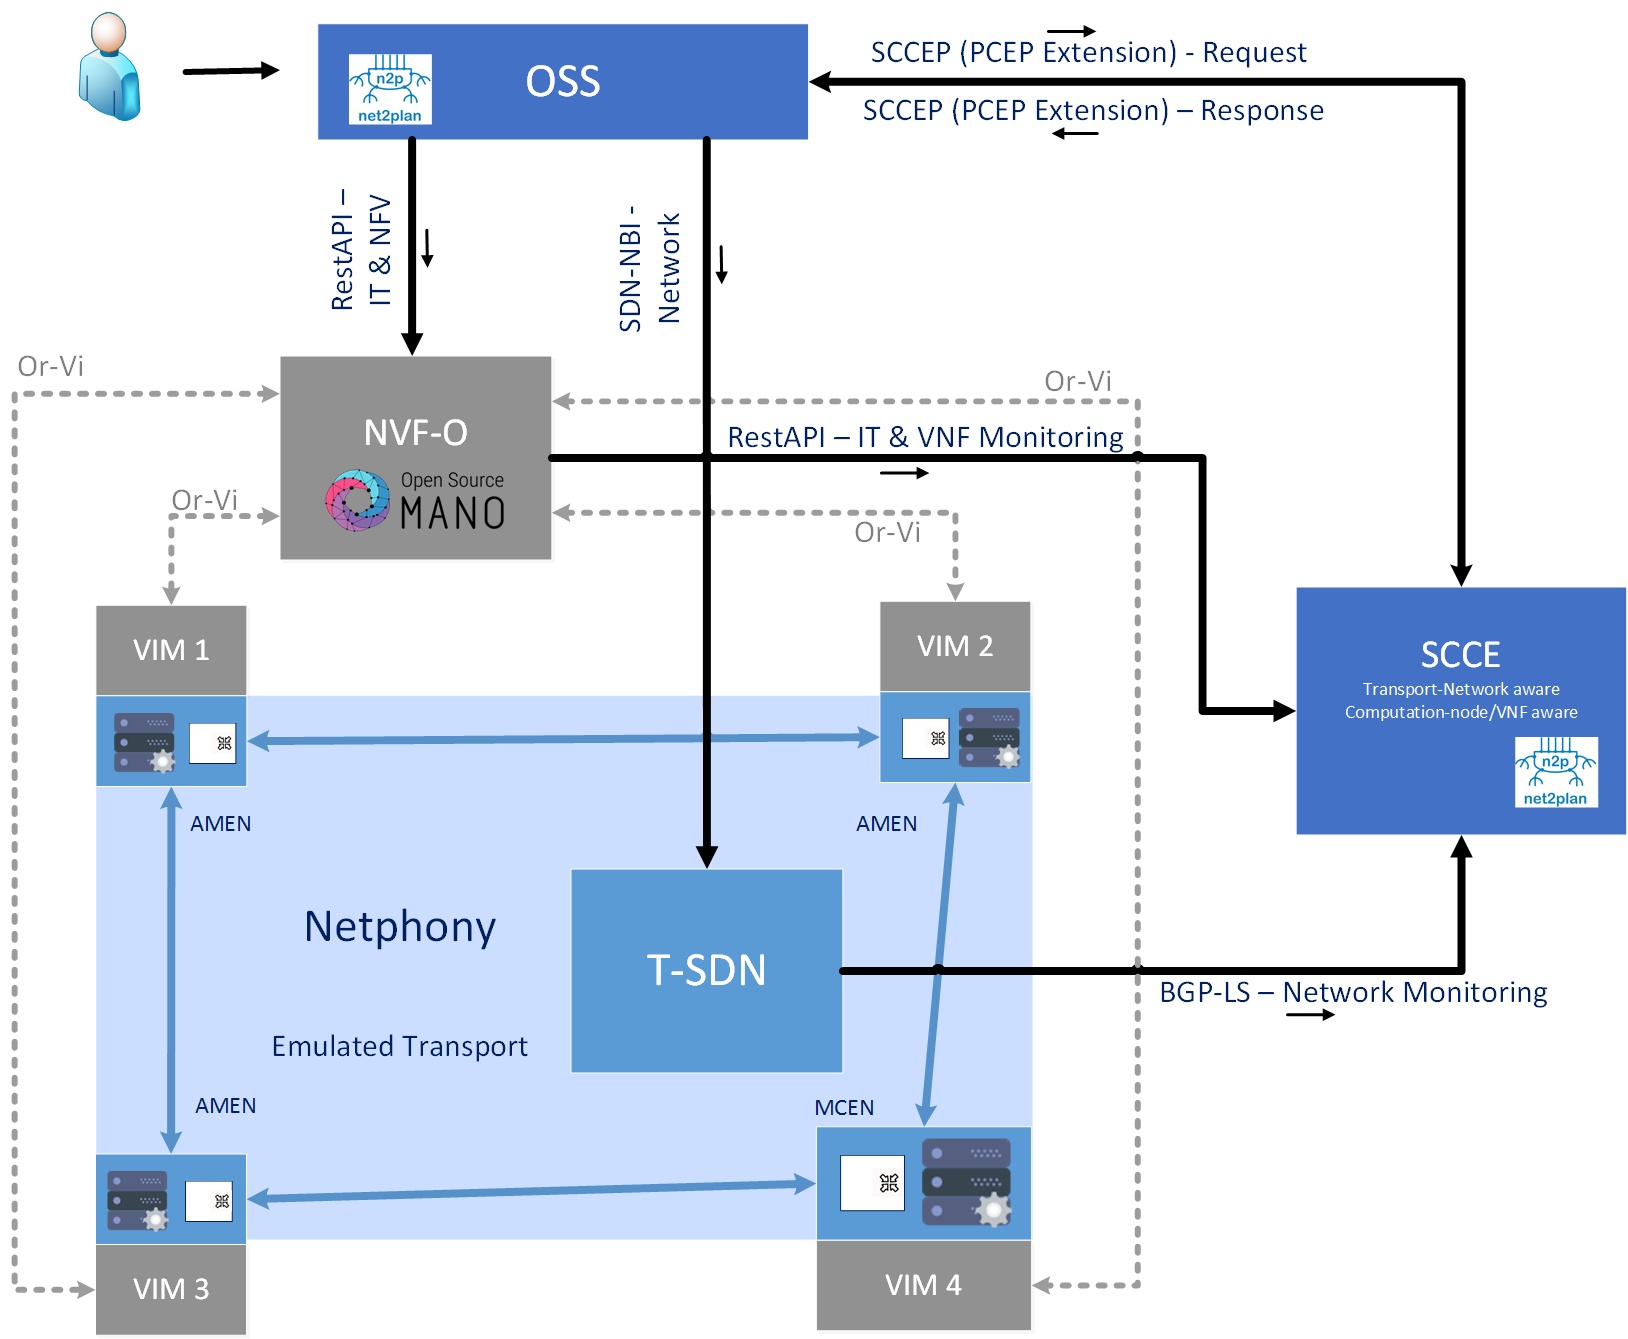
\includegraphics[width=13cm]{diseño}
	\caption{Original schema}
\end{figure}
\section{Previous Settings}

To a proper behavior of the demonstration it is mandatory to accomplish some previous steps to configure the platform before starting the demo. 

\begin{enumerate}
	\item Install and configure the given VIMs, one OpenStack (devstack) per node (different physical machines). Internet access is needed. 
	\item Install Open Source MANO to provide the virtualization platform management and Net2Plan in the same machine (e.g. laptop).
	\item All components have to be connected to the same switch and with Internet access. See figure 2:
	
	\begin{figure}[h!]
		\centering
		\label{fig:workflow}
		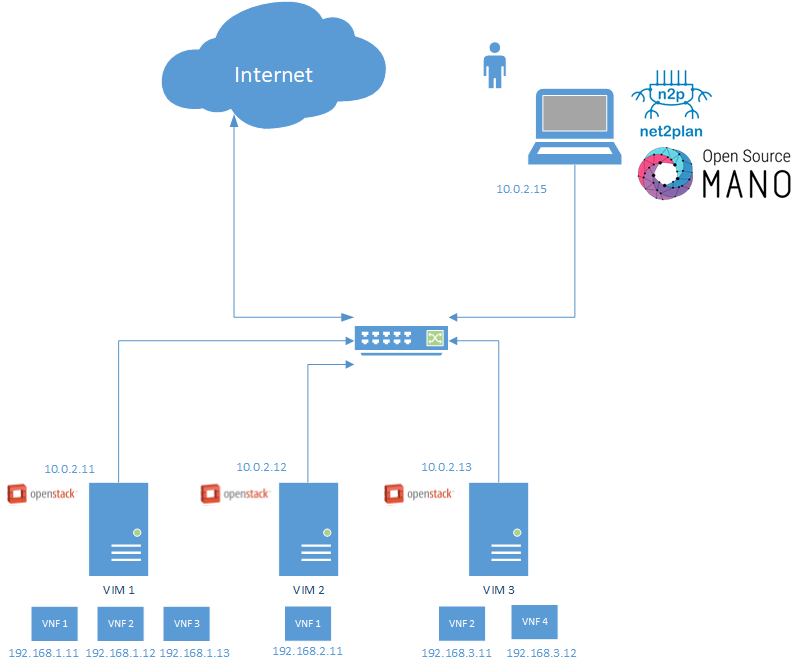
\includegraphics[width=12cm]{workflow}
		\caption{Demonstration schema}
	\end{figure}
	
	\item For simplicity, we assume one VNF per NSD
	\item All the NSDs have to be preconfigured and uploaded in OSM, send the VNF catalog to Net2Plan, Via OSMClient.
	\item Net2Plan requires the information about the total available resources (CPU, RAM, HD, instances) in the VIMs to Net2Plan, via OpenStack4J library.
	\item A User interface is designed in Net2plan in order to emulate the OSS behavior.
	\item Transport network will be emulated by Netphony or Net2plan.
\end{enumerate}

\section{Workflow}

	\begin{enumerate}
		\item A user requests a service chain demand via Net2plan GUI. To build a service chain demand, the user should select the following features. (More information in Appendix A) :
		\begin{itemize}
			\item Initial and destination nodes
			\item A sorted sequence of VNF to traverse
			\item Traffic (bandwidth) to satisfy
		\end{itemize} 
		\item Net2plan runs an optimal algorithm to allocate resource in order to satisfy the service chain.
		\begin{itemize}
			\item For simplicity, we assume an instance is only used by one service chain accomplishment. In other words, once the optimal algorithm is finished, the resulting VNFs have to be created in the corresponding VIMs.
			\item Assuming that there is $N$ VNFs and VIM$_x$ the location chosen by the algorithm to place each instance, Net2plan send a request to OSM to instantiate each VNF$_n$ in its VIM$_x$ (OSMClient).
			\item OSM creates the new virtual machine (vm$_n$) in the VIM$_x$. We have two options to place the vm$_n$ within VIM$_x$: (i) in a preconfigured internal network linked to the virtual router that are previously connects the internal network to the provider public network, or (ii) in a automatically created network, in this last option Net2Plan orders the VIM$_x$ to create an interface in the virtual router to link the new VNF internal network and the public OpenStack network (via OpenStack4J).
			\item Net2plan requests OpenStack to assign a floating IP to the VNF$_n$ to provide external access (via OpenStack4J).
		\end{itemize} 
	
		\item In the next step, Net2plan establishes a connection (e.g. ssh, a new module/class has to be developed in N2P) between the origin and destination nodes through the sorted VNFs and send traffic (e.g. a script or file). As a reminder, the connection has to follow the aforementioned service chain features: 
		\begin{itemize}
			\item IP addresses of the origin and destination nodes.
			\item Floating IP addresses of the VNFs to traverse.
			\item A file to send which models traffic.
		\end{itemize} 
	
		To solve this issue, we assume two different options: see Fig. 3
	
		\begin{figure}[h!]
			\centering
			\label{fig:workflow_2}
			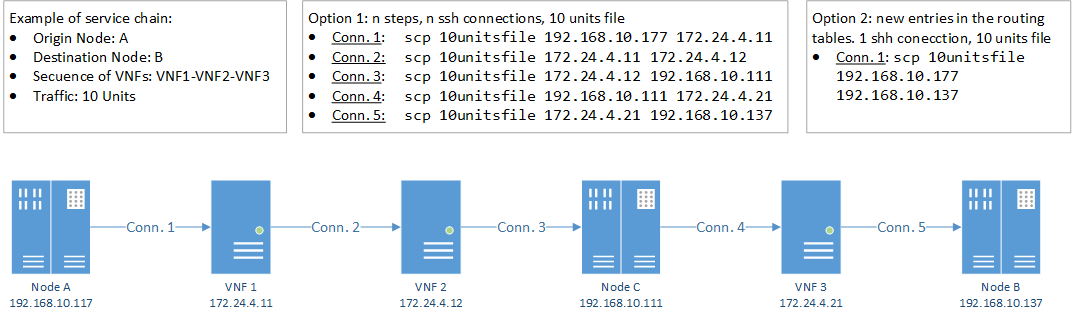
\includegraphics[width=14cm]{workflow_2}
			\caption{Transmission schema}
		\end{figure}
	
		\item After the allocation, Net2plan stores the occupied resources in the model. 
	\end{enumerate}

\newpage

\appendix

\large{\textbf{Appendix A - Net2Plan GUI Customization}}

 A user requests a service chain demand via Net2plan GUI. To build a service chain demand, the user should select the following features :
 
 \begin{figure}[h!]
 	\centering
 	\label{fig:workflow_3}
 	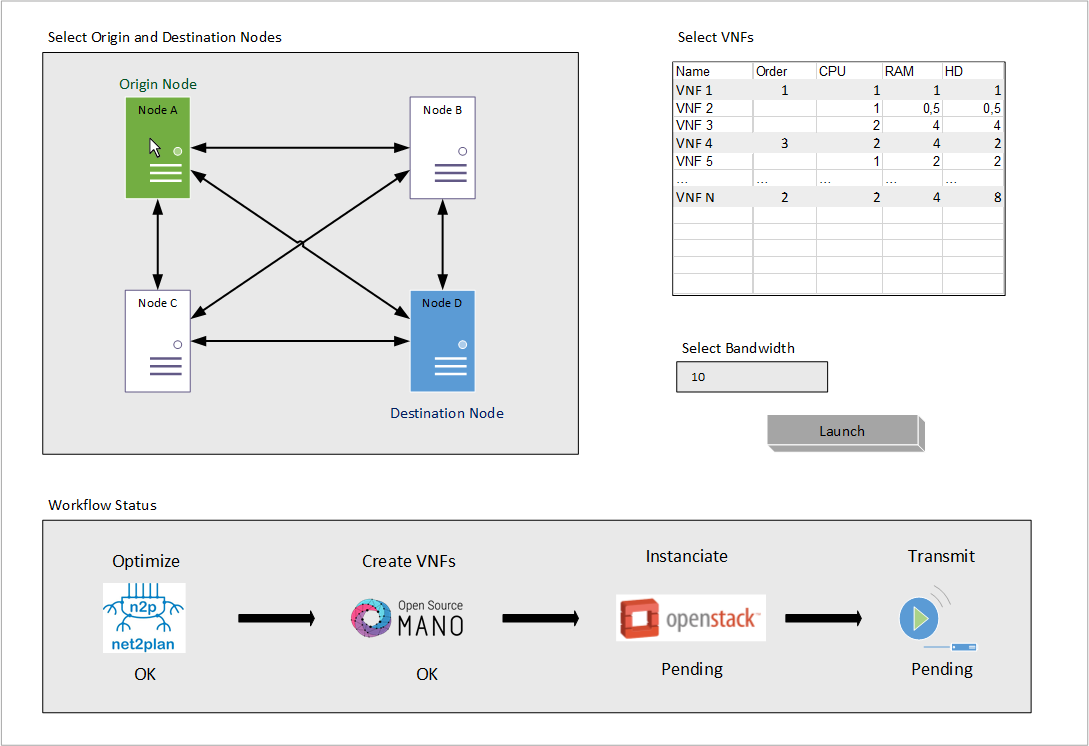
\includegraphics[width=12cm]{workflow_3}
 	\caption{Net2Plan Graphic User Interface}
 \end{figure}
 
 
\begin{itemize}
	\item User can select the initial and destination nodes from the available ones. 
	\item A table with the available VNFs will be shown in order to choose a sorted sequence of VNF to traverse by the user. 
	\item Also, the user can define the traffic (bandwidth) to satisfy
	\item A launch button to execute the service chain satisfaction demo will be clicked to start the process.
	\item To a better overview of the process, there will be a panel where displays the main steps of the workflow and its status.
	\item Finally, if the process is ended without any problem, a small windows noticing the success of the allocation will be shown and also the resources in the Net2plan object will be updated (Demand, Links, Nodes...)
\end{itemize} 


\end{document}
